\documentclass[14pt]{article}
\usepackage[utf8]{inputenc}
\usepackage{amsmath}
\usepackage{graphicx,changepage}
\usepackage{xcolor}
\newcommand\todo[1]{\textcolor{red}{#1}}
\title{LegendOfBluespec}
\author{kr469 }
\date{October 2021}

\begin{document}

\maketitle

\section{Core loop of Bluespec}
    In Bluespec all computation is done in form of rules. Each cycle we will take a subset of all rules that we are going to execute in this cycle, rule is fired (executed) in cycle only if it's ready (or will be ready) and it's not conflicting with other rules (If this happens compiler must issue a warning, and picks arbitrary rule to fire from subset of conflicting rules). Each rule can fire at most one time per cycle. For rule to be ready to fire it needs it's implicit and explicit conditions to be true. Rule can be fired in a cycle even if it's not ready at the start of cycle, for example if you add item on an empty queue and then pop can happen in same cycle.\\
    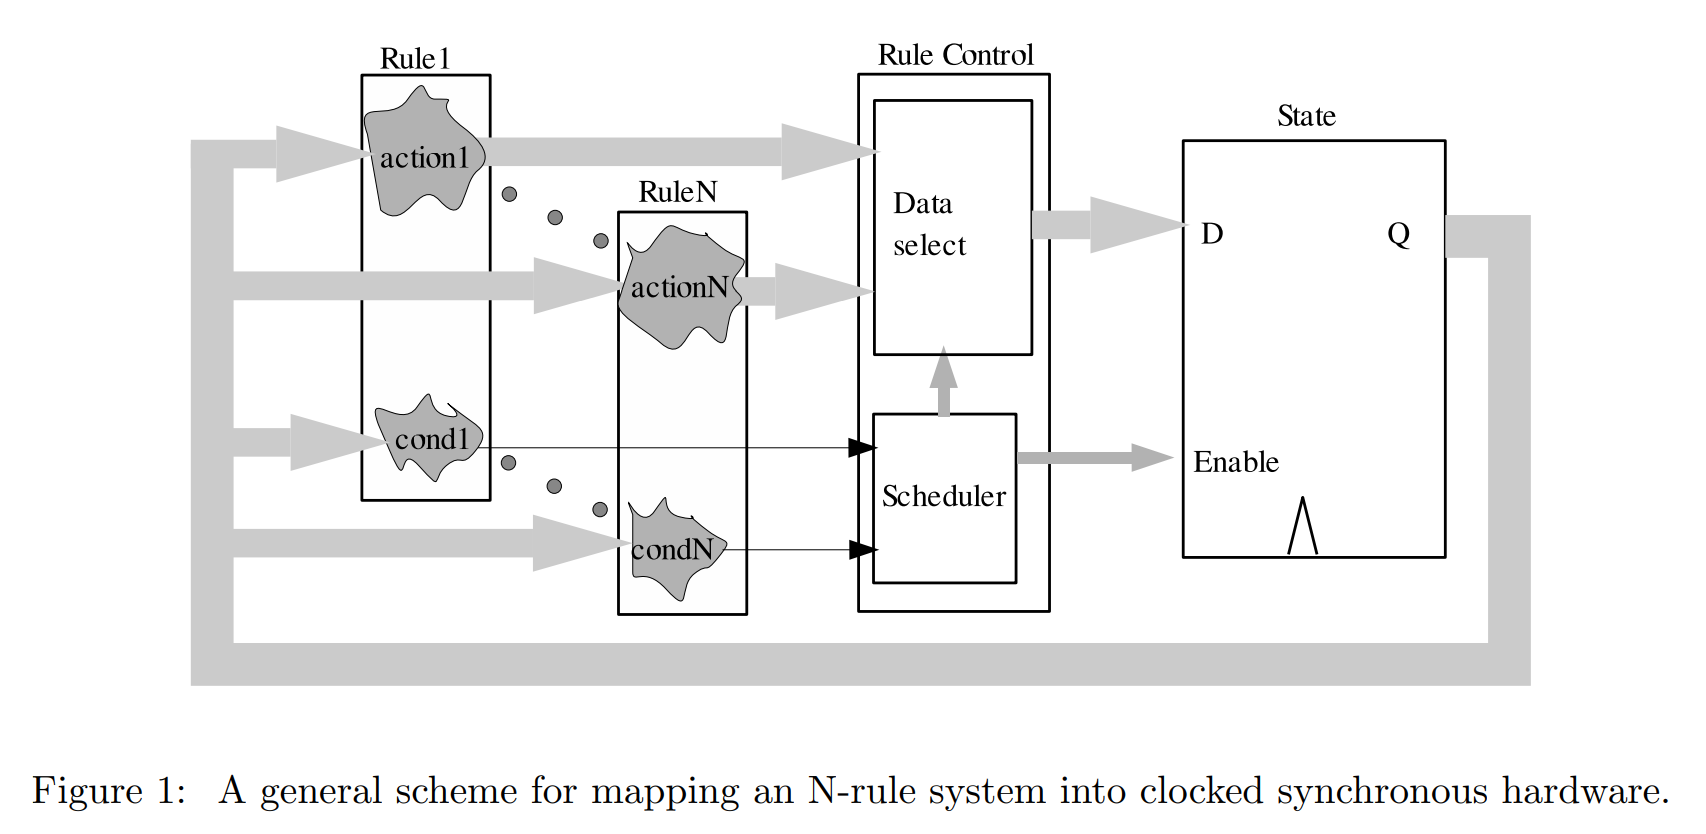
\includegraphics[width=\textwidth]{Rulemapping.png}
    \begin{verbatim}
        
        TODO: piece of Bluespec with module using fifo and other rule
         explaining types of conditions.
        
    \end{verbatim}

\section{Types}
    In Bluespec we can enounter types in 4 categories:
    \subsection{Bit Types}
        This is most common category and contains evey type that is ment to represent data like Int, Bit , Tuples. They are synthesiazable and can store data, during a cycle.
    \subsection{Non-Bit types}
        Those are things like Integer, Real , String that are ment to be used for debug or polymorphism. Most important difference is that you can't syntheside those types so it needs to be possible to know theris values at elaboration.
    \subsection{Interface types}
        This set of types are ment to represent implementation independed sets of functions exposed by a module, or subinterfaces. Here we will find stuff like FIFO intersce with Actions push and pull, or something like Reg (which is interface of an register).
    \subsection{Compiler types}
        Those are things like Action, ActionValue,Rules which are more of a keywords rather than types, and they are used to distinguish functions that are Rules(they can't be called), from Actions which can be called and ActionValues which are functions that return Values.

\section{Interfaces}
    In Bluespec, all modules need to have interfaces. (If it's a top-level module, it can have interface $Empty$). Those interfaces provide a framework for communication between modules. They are like structs that contain only methods or sub-structs. Interfaces can be polymorphic, and we will use this fact to create interfaces that allow for translation between interfaces. A common example would be polymorphic FIFO that can store any type. What's important is that this polymorphism makes it \todo{unsyntesiable}, and its exact type needs to be resolved before a module with such type can be synthesized.
    \\
    TODO : I might add grammar for defining an interface from reference guide.  

\section{Typeclasses}
    Typesclasses in Bluespec are used to group types that contain specific set of functions, like all Bit types are convertable to bit vectors or Arith on which arithmetics are defined.

\section{Provisios}
    In Bluespec there is notion of Provisios they are used to restrict what types can be used in given place. \todo{list places where provisos can appear in} Example use or proviso would be to ensure given type is of certain typeclass so arthmetic operations can be used with it or that it's length in bits is within certain range.
    
\section{Bluetcl}
    Here I will explain what can be extracted from Bluetcl.
    For me most important will be extracting interfaces and functions for module creation.
    To do this I have written down grammar (it's currently in type.lark but I will paste it at some point here).
    
\section{GetPut and other libraries}
    GetPut is library used to make it easier to connect modules,
    but because it is written using normal type system it therore it should be possibe to generalize and handle them via main algorithm without special exception.

\section{System Verilog}
    Using respective compiler flags, one can compile Bluespec to Verilog, and one can add Verilog inserts into Bluespec. Because of this, I will focus only on support for Bluespec as there is available tooling to make my tools work in Verilog projects with Bluespec inserts.

\section{Toolchain}
    \begin{enumerate}
        \item User either starts with .bsc files that needs to be complied to .bo pacages using Bsc.
        \item User feeds .bo/.ba pacages to python libary.
        \item Library uses commands in Bluetcl to extract functions for creating modules, and interfaces of those modules. This information is then cashed.
        \item If GUI is available, then GUI is fed data about known modules and exposes possible modules to the user. Then user creates JSON configuration using this GUI, what might happen underneath is following with steps bellow to immidetly give user feedback about stuff like correctness of values according to the provisos which will be checked only during compliation as they are not exposed in pacages. 
        \item User then feeds library with JSON topmodule configuration file.
        \item Using this file .bsv file is produced containing code of this toplevel module.
        \item This then can be compled using bsv complier. 
    \end{enumerate}
    \todo{Write section about how GUI will also contain tools for debuging and interactivity}

    Tool chain / Pipeline of the library. 
    \begin{enumerate}
        \item Pacages are found using pythons os library. 
        \item For each pacage we find its dependencies
        \item \todo{check if loading packages to bluetcl needs to be done in order}
        \item For each pacage library performs exploration procedure to find all types and functions.
        \item All outputs of bluetcl are red using lark parser. 
        \item Then my algorithm will take care of parsing data from those parse trees. 
        \item For each interface , and module I will try to create coresponding class in python. 
        \item If this is done correctly then I will be able to ensure typing correctness via pythons typing system. 
        \item JSON will be read using some python library.
        \item After all information is accquired I will just instnatiate python object representing toplevel module. 
        \item This object will then have function that converts it into Bluespec code via some tree exploration algorithm.
        \item Such code will need fluff that added at this stage. 
        \item Code is then save to file. 
        \item Library then calls complier to make sure produced code complies. 
        \item In case of errors, due to violating provisos library reports them to user. 
        \item I'm considering currently reporting some of those errors also directly in JSON so it's easy for users to find places that need modifcation. 
    \end{enumerate}


\end{document}
